% !TeX root = thesis_main.tex
% ---------------------------------------------------
% ----- Main document of the template
% ----- for Bachelor-, Master thesis and class papers
% ---------------------------------------------------
%  Created by C. Müller-Birn on 2012-08-17, CC-BY-SA 3.0.
%  Last upadte: C. Müller-Birn 2015-11-27
%  Freie Universität Berlin, Institute of Computer Science, Human Centered Computing. 

\documentclass[pdftex,a4paper,12pt,DIV=calc,BCOR5mm,ngerman,twoside,smallheadings,titlepage]{scrbook}   
% ----- weitere Optionen 
%draft,			% Entwurfsmodus zum Anzeigen zu leerer/voller Boxen 
%DIV=calc
%DIV12,			% Seitengröße (siehe Koma Skript Dokumentation !) 
%BCOR5mm,		% Zusätzlicher Rand auf der Innenseite 
%twoside,		% Seitenränder werden an doppelseitig angepasst 
%fleqn,			% Formeln werden linksbündig (und nicht zentriert) angezeigt 
%titlepage,		% Titel wird in einer 'titlepage' Umgebung gesetzt 
%bigheadings,	% Große Überschriften (normal, small-headings) 
%halfparskip-	% Absatz wird nicht eingerückt, dafür aber um eine halbe Zeile nach unten gerückt
%
%---------------------------------------------------
%----- Packages
%---------------------------------------------------
%
\usepackage[T1]{fontenc} 
\usepackage[utf8]{inputenc}
\usepackage[english]{babel} %\usepackage[english]{babel}  
\usepackage{ae}
\usepackage{biblatex}
\usepackage{bibgerm}

\usepackage{fancyhdr} % Define simple headings 
\usepackage{xcolor}
\usepackage{url}
\usepackage{listings}
%\usepackage{vmargin} % Adjust margins in a simple way
%
\usepackage{amsmath}
%
\usepackage{etoc}
\etocsettocstyle{}{}
\usepackage[pdftex]{graphicx}  
\usepackage{hyperref} % turn all your internal references into hyperlinks
\usepackage{svg}
\usepackage{glossaries}
%\usepackage[pdfstartview=FitH,pdftitle={<<Titel der Arbeit>>}, pdfauthor={<<Autor>>}, pdfkeywords={<<Schlüsselwörter>>}, pdfsubject={<<Titel der Arbeit>>}, colorlinks=true, linkcolor=black, citecolor=black, urlcolor=black, hypertexnames=false, bookmarksnumbered=true, bookmarksopen=true, pdfborder = {0 0 0}]{hyperref}
%
% table settings 
\usepackage{booktabs}  
\usepackage{tabularx}  
\usepackage{rotating}
\usepackage{longtable}
\usepackage{pdflscape}
\usepackage{multirow} %multi row
\usepackage{rotating} %for rotating table
% Diagrams and drawing

\usepackage{tikz}
\usetikzlibrary{shapes.geometric, arrows, positioning, patterns}
\usetikzlibrary{fit,backgrounds}
%
%---------------------------------------------------
%----- PDF and document setup
%---------------------------------------------------
%
\hypersetup{
	pdftitle={How does an editor for dynamic resources for users with different levels of expertise look like and how can it be conceptualized and implemented within the constraints of an exisiting ecosystem?},  % please, add the title of your thesis
    pdfauthor={Matthias Kind},   % please, add your name
    pdfsubject={Bachelor thesis, Institute of Computer Science, Freie Universität Berlin>}, % please, select the type of this document
    pdfstartview={FitH},    % fits the width of the page to the window
    pdfnewwindow=true, 		% links in new window
    colorlinks=false,  		% false: boxed links; true: colored links
    linkcolor=red,          % color of internal links
    citecolor=green,        % color of links to bibliography
    filecolor=magenta,      % color of file links
    urlcolor=cyan           % color of external links
}
% 
%---------------------------------------------------
%----- Customize page size
%---------------------------------------------------
\usepackage[top=3cm,right=3cm,bottom=4cm,left=4cm]{geometry}    
%
%---------------------------------------------------
%----- Customize header and footer\pagestyle{fancy} 
%---------------------------------------------------

% ---------- listings languages

\definecolor{eclipseStrings}{RGB}{42,0.0,255}
\definecolor{eclipseKeywords}{RGB}{127,0,85}
\colorlet{numb}{magenta!60!black}

\lstdefinelanguage{json}{
    basicstyle=\normalfont\ttfamily,
    commentstyle=\color{eclipseStrings}, % style of comment
    stringstyle=\color{eclipseKeywords}, % style of strings
    numbers=left,
    numberstyle=\scriptsize,
    stepnumber=1,
    numbersep=8pt,
    showstringspaces=false,
    breaklines=true,
    string=[s]{"}{"},
    comment=[l]{:\ "},
    morecomment=[l]{:"},
    literate=
        *{0}{{{\color{numb}0}}}{1}
         {1}{{{\color{numb}1}}}{1}
         {2}{{{\color{numb}2}}}{1}
         {3}{{{\color{numb}3}}}{1}
         {4}{{{\color{numb}4}}}{1}
         {5}{{{\color{numb}5}}}{1}
         {6}{{{\color{numb}6}}}{1}
         {7}{{{\color{numb}7}}}{1}
         {8}{{{\color{numb}8}}}{1}
         {9}{{{\color{numb}9}}}{1}
}

% ----------


\pagestyle{fancy}

\bibliography{references.bib}

\fancyhf{}  % delete all existing header formating

\fancyhead[LE]{\leftmark}  % represent the current chapter heading in uppercase
\renewcommand{\chaptermark}[1]{ % adapt the shown chapter name: show it in lower case and with chapter number 
\markboth{\thechapter.\ #1}{}}   

\fancyhead[RO]{\rightmark}   % % represent the current section heading in uppercase 
\renewcommand{\sectionmark}[1]{% adapt the shown section name: show it in lower case and with section number 
\markboth{\thesection.\ #1}{}}

\renewcommand{\headrulewidth}{0pt} % remove lines from header
\renewcommand{\footrulewidth}{0pt} % remove lines from header

\fancyfoot{} % delete all existing footer formating
\fancyfoot[LE,RO]{\thepage} % put page number on the left on even page and right on odd page
%
%---------------------------------------------------      
%----- Settings for word separation  
%---------------------------------------------------      
% Help for separation (from package babel, section 22)):
% In german package the following hints are additionally available:
% "- = an explicit hyphen sign, allowing hyphenation in the rest of the word
% "| = disable ligature at this position. (e.g., Schaf"|fell)
% "~ = for a compound word mark without a breakpoint (e.g., bergauf und "~ab)
% "= = for a compound word mark with a breakpoint, allowing hyphenation in the composing words
% "" = like "-, but producing no hyphen sign (e.g., und/""oder)
%
% Describe separation hints here:
\hyphenation{
% Pro-to-koll-in-stan-zen
% Ma-na-ge-ment  Netz-werk-ele-men-ten
% Netz-werk Netz-werk-re-ser-vie-rung
% Netz-werk-adap-ter Fein-ju-stier-ung
% Da-ten-strom-spe-zi-fi-ka-tion Pa-ket-rumpf
% Kon-troll-in-stanz
}
%
%---------------------------------------------------
%----- Restricting including files   
%---------------------------------------------------
% Only files listed here will be included in the PDF document!
% In order to only partially translate the document, for example for bug-fixing, 
% it might be useful to comment out some of the documents.
% \includeonly{
% title,
% declaration,
% abstract_en,
% abstract_de,
% preface,
% introduction,
% chapters,
% chapters/02-background
% conclusion,
% appendix
% }

\makenoidxglossaries
\loadglsentries{glossary}

%%%%%%%%%%%%%%%%%%%%%%%%%%%%%%%%%%%%%%%%%%%%%%%%%%%%%%
% The content part of the documentent starts here! %%
%%%%%%%%%%%%%%%%%%%%%%%%%%%%%%%%%%%%%%%%%%%%%%%%%%%%%%

\begin{document}
%---------------------------------------------------
%----- Listing and color definition   
%---------------------------------------------------
\definecolor{red}{rgb}{.8,.1,.2}
\definecolor{blue}{rgb}{.2,.3,.7}
\definecolor{lightyellow}{rgb}{1.,1.,.97}
\definecolor{gray}{rgb}{.7,.7,.7}
\definecolor{darkgreen}{rgb}{0,.5,.1}
\definecolor{darkyellow}{rgb}{1.,.7,.3}
\lstloadlanguages{C++,[Objective]C}
\lstset{
		escapeinside={§§}{§§},
        basicstyle=\ttfamily\footnotesize\mdseries,
        columns=fullflexible,% typewriter font look better with fullflex
        keywordstyle=\bfseries\color{blue},
%		identifierstyle=\bfseries,
        commentstyle=\color{darkgreen},      
        stringstyle=\color{red},
        numbers=left,
        numberstyle=\ttfamily\scriptsize\color{gray},
%       stepnumber=5,
%       numberfirstline=true,
        breaklines=true,
%		prebreak=\\,
        showstringspaces=true,
        tabsize=4,
        captionpos=b,
%		framexrightmargin=-.2\textwidth,
        float=htb,
		frame=tb,
		frameshape={RYR}{n}{n}{RYR},
		rulecolor=\color{darkyellow},
        xleftmargin=15pt,
        xrightmargin=4pt,
        aboveskip=\bigskipamount,
        belowskip=\bigskipamount,
		backgroundcolor=\color{lightyellow},
		extendedchars=true,
       	belowcaptionskip=15pt
}

%---------------------------------------------------
%----- Title and declaration   
%---------------------------------------------------
\pagenumbering{alph} % even though, these page numbers are not visible there are necessary to have unique page numbers 
% !TeX root = thesis_main.tex
% ---------------------------------------------------
% ----- Title page of the template
% ----- for Bachelor-, Master thesis and class papers
% ---------------------------------------------------
%  Created by C. Müller-Birn on 2012-08-17, CC-BY-SA 3.0.
%  Freie Universität Berlin, Institute of Computer Science, Human Centered Computing. 
%
\pagestyle{empty}

\begin{titlepage}

\title{
{\small Bachelorarbeit am Institut für Informatik der Freien Universität Berlin}\\
{\small Human-Centered Computing (HCC)}\\
[6ex]
{\LARGE How does an editor for dynamic resources for users with different levels of expertise look like and how can it be conceptualized and implemented within the constraints of an exisiting ecosystem?}}

% Title laternative ideas:
% Building an Editor for Dynamic Resources: Challenges and Opportunities in an Existing Ecosystem
% Creating an Editor for Dynamic Resources within Constraints: A Case Study

\author{
{\emph{\normalsize{Matthias Kind}}}\\
{\normalsize Matrikelnummer: 5338650}\\
{\normalsize matthias.kind@fu-berlin.de}\\ 
[18ex]   
{\normalsize Betreuer: Florian Berger} \\
{\normalsize Erstgutachterin: Prof. Dr. Claudia Müller-Birn} \\
{\normalsize Zweitgutachter: Prof. Dr. Lutz Prechelt}}
\vspace{6ex}
\date{\normalsize Berlin, 1.2.2023}
\maketitle
\end{titlepage}

\include{declaration}

%---------------------------------------------------
%----- Abstracts in English and German   
%---------------------------------------------------
\mainmatter

% !TeX root = thesis_main.tex
% ---------------------------------------------------
% ----- Abstract (English) of the template
% ----- for Bachelor-, Master thesis and class papers
% ---------------------------------------------------
%  Created by C. Müller-Birn on 2012-08-17, CC-BY-SA 3.0.
%  Freie Universität Berlin, Institute of Computer Science, Human Centered Computing. 
%

\chapter{Abstract}

In recent years, the shift from print to digital publishing channels has increased the need for tools that allow publishers to quickly build and configure apps and websites.
\\\\
The goal of this bachelor thesis is to conceptualize, plan, and implement an UI editor for apps and websites used by magazine and news publishers, particularly in Germany and the UK.
The editor was built for a properitary web framework called "Purple Experience" and was developed within the constraints of an existing software ecosystem, which posed challenges and limitations on the design and implementation of the tool.
\\
To gain insights into the needs and workflows of the groups of users who will be using the editor, a variety of HCI methods were applied during the user research phase, including moderated observations and interviews. 
\\\\
The outcome of this research is useful as guidance for future software development projects for internal tools at companies, or in environments where constraints exist but a user base is already in place to provide valuable input and feedback. As a result of the user research phase, an interactive prototype was built using modern web technologies and was deployed to a controlled group of test users. This allowed for quick feedback and fast iteration until the tool was ready for a broader audience.

\textbf{TODO reformulate}
\\
Learned: 
- if existing user base (manageable number): qualtitative research methods seem to provide more value / deeper feedback than quantitative
\\
- if existing products: use tracking etc. to figure out who already uses tools how, as a base line for comparison
\\
- use vizualizations and other methods to sort ideas by multiple dimensions (user value, impl. effort) -> easier to reason what to do next \& to convince other stakeholders
% !TeX root = thesis_main.tex
% LTeX: language=de-DE
% ---------------------------------------------------
% ----- Abstract (German) of the template
% ----- for Bachelor-, Master thesis and class papers
% ---------------------------------------------------
%  Created by C. Müller-Birn on 2012-08-17, CC-BY-SA 3.0.
%  Freie Universität Berlin, Institute of Computer Science, Human Centered Computing. 
%
% \pagestyle{empty}

\addcontentsline{toc}{chapter}{Zusammenfassung}
\chapter*{Zusammenfassung}

In den letzten Jahren hat die Verlagerung von gedruckten zu digitalen Publikationskanälen dazu geführt, dass Verlage Werkzeuge brauchen, mit denen schnell und einfach digitale Plattformen gebaut und konfiguriert werden können.
\\\\
Die vorliegende Bachelorarbeit befasst sich mit diesem Problem, in dem als Fallstudie ein User Interface (UI) Editor für Apps und Webseiten von Magazin- und Nachrichtenverlagen entworfen und implementiert wird.
Der Editor wird für ein proprietäres Web Framework namens \Gls{experience} gebaut, wobei die Limitierungen des existierenden Softwareökosystems berücksichtigt werden müssen.
Dies brachte Herausforderungen und Einschränkungen für das Design und die Implementierung des Tools mit sich.
\\
Um Einblicke in die Bedürfnisse und Arbeitsweisen der Nutzergruppen zu gewinnen, werden in der Benutzerforschungsphase verschiedene Methoden der Human Computer Interaction (HCI)
Methoden angewandt, darunter moderierte Beobachtungen und Interviews.
\\\\
Die Forschungsergebnisse können als Leitfaden für zukünftige Softwareentwicklungsprojekte
Entwicklungsprojekte für interne Tools in Unternehmen dienen.
Zudem können sie nützlich sein, wenn in der Softwareumgebung zwar Einschränkungen gelten, jedoch eine bereits vorhandene Nutzerbasis wertvollen Input und Feedback liefern kann.
Ergebnis dieser Forschungsphase ist ein interaktiver Prototyp unter Verwendung moderner Web-Technologien. Darauf folgend wird de UI Editor einer Gruppe von Testnutzern zur Verfügung gestellt.
Dieser Ansatz, kombiniert mit agiler Softwareentwicklung, ermöglichte schnelle Iterationen und das Sammeln von direktem Feedback vor dem öffentlichen Release.

Es wird aufgezeigt, wie wichtig die Berücksichtigung von HCI-Prinzipien für Brownfield-Softwareentwicklungsprojekte ist, und ich gebe Beispiele, wie diese Prinzipien in einen realen Kontext integriert werden können.  
                                          
%---------------------------------------------------
%----- Directories   
%---------------------------------------------------

\pagenumbering{roman}

\tableofcontents
\setcounter{tocdepth}{3}   % reduce the included sections in the table of content

\listoffigures

%---------------------------------------------------
%----- Main part
%---------------------------------------------------
\pagenumbering{arabic} 
\pagestyle{fancy} 

% !TeX root = thesis_main.tex
% ---------------------------------------------------
% ----- Introduction of the template
% ----- for Bachelor-, Master thesis and class papers
% ---------------------------------------------------
%  Created by C. Müller-Birn on 2012-08-17, CC-BY-SA 3.0.
%  Last upadte: C. Müller-Birn 2015-11-27 
%  Freie Universität Berlin, Institute of Computer Science, Human Centered Computing. 
%
\chapter{Introduction}
\label{chap:introduction}

\section{Topic and context}

In the evergrowing world of software companies, many once startups are now in the situation where they maintain a large software ecosystem and have complcated dependencies of other services or users,
but still want to improve their systems by developing new components and tools.

This poses the challenge of improving the software from aspects like user expeirence, scalability and maintainability while beeing restricted by the ecosystem.
Greenfield development, as it is taught for the majority of books, can't be applied freely without breaking existing features or behaviours.
Thus, applying HCI methods for user research and user experience-focused design might needs to be approached in a diffrent way then during greenfield development.
Also, the common problem of tight deadlines and limited resources allocated by managers tend to lead to premature releases and unstable software.
Instead of developing software to maximize the three HCI factors \textbf{See HCD principles / factors src, anme the tree?} for the actual users, often ideas from individual stakeholders like the executive floor are realized without adding real value.

On the other hand, having an exsisting user base which works with exisiting tools is a great fundament to evaluate what ''real users'' need. So HCI methods applied to them can yield more helpful and focused results. \textbf{rephrase}

Many of the resources or literature about HCI seem to assume a mostly free degree while developing new tools, and also assume a wide user base with diverse demographic features \textbf{is this valid engilsh?}.
\\
\textbf{List literature srces that dont speak about brownfield development?}
\textbf{Find a contra example that does cope with brownfield}
	

\section{Goals of this work}
\begin{itemize}
	\item Was sind die mit dieser Arbeit verfolgten Ziele? Welches Problem soll gelöst werden?
	\item Eine Beschreibung der ersten Ideen, der vorgeschlagene Ansatz und die aktuell erreichten Resultate 
	\item Eine Beschreibung, welchen Beitrag die Arbeit leistet, um das vorgestellte Problem zu lösen
	\item Eine Diskussion, wie die vorgeschlagene Lösung sich von bestehenden unterscheidet, was ist neu oder besser?
\end{itemize}

The goal of this thesis is to implement a new software product, an UI Editor for Apps \& Websites of digital publishing customers,
which is embedded in an existing software ecosystem. During that process, diffrent HCI methods get applied and  

\section{Procedure for the research and implementation}

While writing the software and thesis, I followed the an software design process described in \cite[p. 104]{LearnHCI:2020ys}.
There, the process is divided into a ''Idea'' phase using design thinking, lean ux for first prototypes and then agile development (in my case a relaxed SCRUM version).
Abstractly it looks as following:

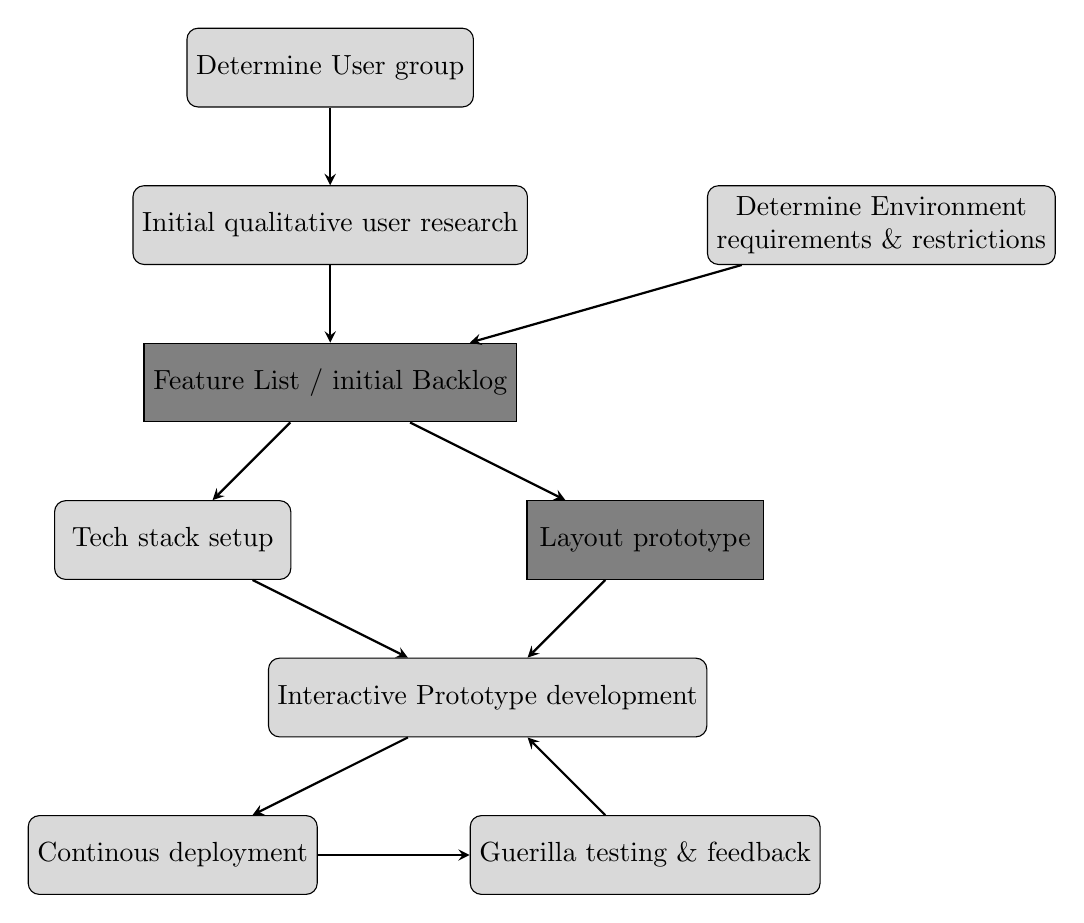
\begin{tikzpicture}[node distance=2cm]
  \tikzstyle{round} = [rectangle, rounded corners, minimum width=3cm, minimum height=1cm,text centered, draw=black, fill=gray!30]
  \tikzstyle{rect} = [rectangle, minimum width=3cm, minimum height=1cm,text centered, draw=black, fill=gray]
  \tikzstyle{arrow} = [thick,->,>=stealth]

  \node (dug) [round] {Determine User group};
  \node (interview1) [round, below of=dug] {Initial qualitative user research};
  \node (denv) [round, right of=interview1, xshift=5cm, align=center] {Determine Environment\\requirements \& restrictions};
  \draw [arrow] (dug) -- (interview1);
  \node (bl) [rect, below of=interview1] {Feature List / initial Backlog};
  \draw [arrow] (denv) -- (bl);
  \draw [arrow] (interview1) -- (bl);
  \node (tech1) [round, below of=bl, xshift=-2cm] {Tech stack setup};
  \node (layout) [rect, right of=tech1, xshift=4cm] {Layout prototype};
  \draw [arrow] (bl) -- (tech1);
  \draw [arrow] (bl) -- (layout);
  \node (proto) [round, below of=tech1, xshift=4cm] {Interactive Prototype development};
  \draw [arrow] (tech1) -- (proto);
  \draw [arrow] (layout) -- (proto);
  \node (deploy) [round, below of=proto, xshift=-4cm] {Continous deployment};
  \draw [arrow] (proto) -- (deploy);
  \node (feedback) [round, right of=deploy, xshift=4cm] {Guerilla testing \& feedback};
  \draw [arrow] (deploy) -- (feedback);
  \draw [arrow] (feedback) -- (proto);
\end{tikzpicture}
  


% \section{Aufbau der Arbeit}
% \begin{itemize}
% 	\item Welche Schritte werden durchlaufen, um die Ziele zu erreichen?
% 	\item An dieser Stelle ist beispielsweise eine Grafik hilfreich, um den Aufbau der Arbeit und welche Ergebnisse/Erkenntnisse wo genutzt werden, zu visualisieren. 
% 	\item Ebenfalls sollten noch Anmerkungen zur Gestaltung der Arbeit gegeben werden, vor allem, da in vielen deutschen Arbeiten englische Fachbegriffe verwendet werden. Ein solcher Text könnte folgendermaßen lauten: 
% 		\begin{itemize}
% 			\item ``Abschließend sind hier noch eine Anmerkungen zur Gestaltung der vorliegenden Arbeit. Für die im Folgenden verwendeten personenbezogene Ausdrücke wurde, um die Lesbarkeit der Arbeit zu erhöhen, die männliche Schreibweise gewählt. Des Weiteren werden eine Reihe von englischen Bezeichnungen verwendet, um einerseits dem interessierten Leser das Studium der häufig vorliegenden englischen Originalliteratur zu erleichtern oder andererseits bestehende Fachbegriffe nicht durch die Übersetzung zu verfälschen. Diese Begriffe sind vom herkömmlichen Text in kursiver Schrift unterschieden.''
% 		\end{itemize}
% \end{itemize}

% \begin{figure}[!ht]
% 	% Mit [!h] wird die Position der Grafik bestimmt. So bedeutet h=here und mit dem "!" (Ausrufezeichen) wird dieser Befehl verstärkt. Weitere Möglichkeiten sind : t=top und b=bottom. Zumeist wird angegeben, in welcher Reihenfolge LaTeX versuchen soll das Bild einzufügen, z.B. [!htb].
% 	\centering
% 		\includegraphics[width=0.95\textwidth]{pics/structure.pdf}
% 	\caption[Beispiel einer möglichen Darstellung zum Aufbau der Arbeit]{Beispiel einer möglichen Darstellung zum Aufbau der Arbeit (vgl. Beschreibung Abschnitt  \ref{chap:chapters}).} 
% 	% Mit Hilfe von caption wird die Bildunterschrift erzeugt. Der Text in geschweiften Klammern erscheint im Text, während der Text in eckigen Klammern sich dann empfiehlt, wenn die Beschreibung besonders lang ist, denn diese wird dann im Bildverzeichnis verwendet. Diese Kurzbeschreibung kann auch weggelassen werden. 
% 	\label{fig:structurethesis}
% \end{figure}
% !TeX root = ../thesis_main.tex

% ---------------------------------------------------
% ----- Chapters of the template
% ----- for Bachelor-, Master thesis and class papers
% ---------------------------------------------------
%  Created by C. Müller-Birn on 2012-08-17, CC-BY-SA 3.0.
%  Freie Universität Berlin, Institute of Computer Science, Human Centered Computing. 
%
\chapter{Theoretical background}
\label{chap:background}

Before discussing the design and implementation of the UI Editor, it is necessary to provide a brief overview of the applied parts of HCI and the specific context, challenges and opportunities in which the UI Editor was developed.
% 

\section{Applied human-computer interaction methods}

This section concretizes the HCI aspects of this work and describes how and why the subject is approached from a not so common point of view.
HCI is a complex topic with a long list of available methods and even more ways to adapt them to a concrete project, so it is impossible to cover all aspects.
The UI Editor development faced challenges in integrating with an existing ecosystem and meeting technical requirements in a \gls{brownfield} project.
In my opinion, technical requirements face only limited coverage in HCI literature.
Therefore, the focus was set on them during this case study.
\\
To determine the initial functional requirements, qualitative user research methods like moderated observations (\ref{subsec:modobs}) and interviews (\ref{subsec:interview}) were chosen to be applied in an initial Design Thinking phase.
While quantitative research methods were also used to get insights during the testing phase, the decision was made against using them for this phase.
The available user base was small enough to get meaningful and representative statements only from qualitative research.
A questionnaire would either be too long or not provide enough helpful insights.
\\
Furthermore, the two concepts "SMART goals" and "three major factors of HCI" were used as foundation and guidelines during the process, which is described in chapter \ref{chap:research} in more detail.

\section{Project specific background}

In the following the functional and technical requirements are described to gain an understanding of the application domain.

\subsection{Functional}

The publishing houses respectively their digital departments (in the following \textit{customer}) purchase the license for an app or website (in the following just \textit{app}, as there is not much difference besides the end medium).
Then, they can import content via multiple ways into the system, or the editors write the content directly inside the tools provided as \Gls{saas}.

\begin{figure}[h!]
  \includegraphics[width=\textwidth]{pics/purple-abstract.drawio.png}
  \caption{Use case diagram: interactions from publishers, readers and frontend developers with the system TODO: position}
  \label{fig:usecase1}
\end{figure}

The UI Editor fits into the use case "Per App configuration \& style" (see fig. \ref*{fig:usecase1}), with which mostly Frontend Developers and Project Managers from Sprylab as well as some external customer's IT Admins will interact. The goal is to lower the editing burden as much as possible, so that more of the configuration can be handed off to external customers while also improving usability for the developers of the company.

\subsection{Technical}

The UI Editor will be implemented within the context of the proprietary web framework Purple Experience which is built on top of Angular.
This framework allows complete configurability through JSON files, including routing, rendering of different components, connecting data sources, loading assets and styling the page with CSS.
These configs and assets are stored in a per-app file system called \label{def:DynamicResources} dynamic resources.
\\\\
Dynamic resources are individually managed and loaded for every app. This way, on mobile phones the end users download a native core app, which in turn just downloads the dynamic resources and executes the angular app with the configs provided from the resources.
Similar, when an end user requests a website, the backend server just looks up the dynamic resources matching this app's domain and renders the website using that config.
As a result all customers can share the same server instance(s) in case of websites, or at least don't require extra native sourcecode changes per app.
\\
In addition, there are preview and live resources for every app, so that changes can be tested before they are released to the end users.
\begin{figure}[h!]
  \includegraphics[width=\linewidth]{pics/experience_resources.drawio.png}
  \caption{Sprylab preview and live dynamic resources for two imaginary apps}
  \label{fig:dynres}
\end{figure}
\\
Working with large and deeply nested JSON files quickly becomes convoluted.
Manual handling of ZIP files, including modification of assets, repackaging, and the subsequent risk of introducing errors, is a labor-intensive and error-prone workflow.
TODO ref to \ref{fig:viewexample}
\\
As a base for making editing of these configuration JSON files easier, Purple Experience generates JSON Schema files directly from the interfaces in the source code for every released version.
JSON Schema is a specification and a declarative language ''that allows you to annotate and validate JSON documents.'' (Retrieved 11th January 2023, from \url{https://json-schema.org/}).
The use of UI elements generated from JSON Schemas allows for direct validation of user input and prevents the entry of invalid states.

At Sprylab exists a tool called "Storefront Editor", which is the predecessor for this new UI Editor.
It uses an open source software called \textit{Json Editor} (\url{https://github.com/json-editor/json-editor}), which is an implementation of the UI elements for JSON validation mentioned above.
In chapter \ref{chap:research}, the state of the JSON Editor for that use case is evaluated and the positive aspects and approaches which I reused for the new editor are generally outlined.
Furthermore, features are described which are missing, or the interview candidates noted as confusing, not working or slowing down their work.

\begin{figure}[h]
  \lstset{language=json,basicstyle=\footnotesize,numbers=left,showstringspaces=false,frame=single}
  \begin{lstlisting}
{
  "type": "view",
  "path": "/newsstand",
  "content": [
    {
      "type": "list",
      "content": {
        "type": "issue"
      },
      "dataSource": {
        "type": "issue",
        "filter": {
          "purchased": {
            "value": true
          }
        }
      }
    }
  ]
}
  \end{lstlisting}
  \caption{Simplified example of a view configuration showing purchased issues}
  \label{fig:viewexample}
\end{figure}

Figure \ref{fig:viewexample} shows a minimal example of a view configuration with which the Purple Experience could render a simple page.
The page would be accessible under the domain of the app; for example \textit{https://app1.com/newsstand} and show a list of issue components.
The data for these components is taken from the data source of type \textit{issue} which filters the published content for issues that are purchased by the current user. 
\\
In public apps, the configs are more advanced with conditionals declaring when components are rendered or filters are applied, event handlers when a user interacts with an element and many more functionalities that are modeled through the JSON Schema.


\section{Related Work}

TODO
\include{chapters/related_work}
% ---------------------------------------------------
% ----- Chapters of the template
% ----- for Bachelor-, Master thesis and class papers
% ---------------------------------------------------
%  Created by C. Müller-Birn on 2012-08-17, CC-BY-SA 3.0.
%  Freie Universität Berlin, Institute of Computer Science, Human Centered Computing. 
%
% TODO remove 2 - to use auto numbering
\chapter{User research and analysis}
\label{chap:research}


% Due to the limited size of the user group, the goal was not to gain <TODO> with high diversity of their demographics, but to have information saturation from fewer but more valuable insights into peolpe with diffrent workflows.

Cites:
\begin{itemize}
  \item \cite{Ross:2016} why companies dont conduct user research
\end{itemize}

Over ten years after the publication of Tomer Sharon's book ''It's our Research'', the listing of qoutes in the introduction about user research in software companies still feel as relevant as ever.
\\
''Yeah, but this study will delay our launch date.'', ''Yeah, but we can't learn much from only five participants.'', ''Yeah, but research sounds so academic.'' \cite[p. 4]{Sharon:2012mk} are only some of the statements that according to Sharon are often heard in software companies when discussing if UX research should be conducted.
\\
The common pressure from different stakeholders often leads to quick implementation of features and workflows without first investing time to figure the user's needs out, which may be faster in the beginning, but can badly impact the user's acceptance of the product due to cumbersome and slow workflows,
in the worst case leading to the user not using the product anymore.

To counteract this, it is crucial to conduct and evaluate user research methods, which is what I did for the development of the UI builder.

A starting point for qualitative user research is to define the goals through the help of the SMART criteria, which provide guidelines and formulated goals during research.

For the project, I defined the SMART criteria as following:

\begin{itemize}
  \item \textbf{specfic} - improve the workflow of users modifying dynamic resources for the Purple Experience.
  \item \textbf{measurable} - interviews after testing period concerning working speed, confidence and <TODO Spaß?> when editing resources, automated user tracking
  \item \textbf{assignable} - research and implementation will mostly be conducted by me, with input from CTO \& product owner, connections to external users through customer service team
  \item \textbf{realistic} - new software platform which reacts quicker, prvides more safety regarding errors and is scalable and extensible in the future. Limiting factors are time (as I only have three months for the first phase, including writinh this thesis)
  \item \textbf{time-related} - the new software should have at least the same feature set and be usable by company-internal users until the end of 2022
\end{itemize}

\section{Identifying and categorizing users and user groups}
\label{sec:user-groups}
In order to effectively design and implement the UI editor, it is crucial to understand the needs and preferences of the various users and user groups who will be using the tool.
Therefore, the first step in the user research process was to identify and categorize the different users and user groups who will be using the editor.

In a later chapter (\ref{sec:personas}), I'll build concrete Personas for the different user groups utilizing the information gained from the interviews.
\\
Because we already have existing users that work with the previous editors and other tools from the ecosystem, it was relatively easy to collect a list of internal and extneral users, which either I personally knew or I could write a short message asking about if and how they use existing tools and modify dynamic resources.
I see that this won't be as easy when dealing with a larger user base or primary external customers, when this first step probably requires more effort to collect a user overview upfront.
\\
With a list of many of the users, I started grouping them to understand the characteristics and needs of each user group, through which can ensure that the UI editor is tailored to their specific requirements and can be used effectively by all users\footnote{When I refer to ''all users'', I mean the group of users that are expected to work with the tool. There is an expected technical and domain specific base knowledge that the Editor won't cover}.
\\
I derived the follwoing commomn factors from the users, which made the communication and categorization a lot easier.

\begin{itemize}
  \item \textbf{quantitative usage} There were users who relied on the tools for most of their work, while others like the external customers accessed the tool a few times a year.
  \item \textbf{common tasks} I roughly categorized the common tasks into three groups:
    \subitem \textbf{Heavy configuration} Mostly internal devs used the tools to build new apps and websites from scratch (or derived from exisiting apps), making many modifications, from structural changes to the seperate views, menus, data sources and more, over styling and translating messages to diffrent languages.
    \subitem \textbf{Moderate configuration} Project devs and customer support people copy resources from existing apps and adapt them for new brands, which often includes changing colors and logos, adapting texts or switching authentification flows.
    \subitem \textbf{Small changes} External customers often only use the tools to exchange some ads, translations or logos, which affects a small set of files.
  \item \textbf{expertise} 
  %<kann man bei schlechter software gut erkennen, leute mit viel erfahrung checken sachen, aber ist für neue nicht intutitiv>
    \subitem \textbf{Technical} Depending on the area of education and working time in the web development industry, the expertise about web technologies, languages like CSS and JSON and often also intuition differs between users.
    \subitem \textbf{Domain- and Platform Specific} There is a lot of vocabulary, functionality of the Purple Experience and other systems as well as permutations of configurations that users learn with time.
\end{itemize}

% ... more
\section{Qualitative user resarch}

\begin{itemize}
  \item mix interview / moderated observation
  \item experiences, outcomes, what went good and bad
\end{itemize}

\subsection{Interview}

TODO interview preparation and conduction

\subsection{Moderated observation}

TODO prep and conducting

\section{Quantitaive user research}

Not used survey / questionaire -> lay down reasons why not necessary in that situation

Tracking of user behaviours

- on site using G analytics \& (the other GDPR compliant tracking tool name??)
- using server logs to understand usage patterns

\section{Process and vizualize the outcomes of the initial user research phase}

\subsection{2x2 Opportunity Matrix}

This two-dimensional vizualization of a set of proposed features prooved helpful when prioritizing tasks with other stakeholders,
as it shows the (approximated) cost of implementation as well as the value the feature can have for users.

The matrix I used is a slightly modified adaption from \cite[p. 181]{LearnHCI:2020ys}, replaced the term ''idea originality'' on the x-axis with ''Value''.

\begin{figure}[ht]
	\centering
  \includegraphics[width=\textwidth]{pics/feature_cost_matrix.excalidraw.png}
	\caption{2x2 Opportunity Matrix during the early phases of development}
	\label{fig:opportunitymatrix}
\end{figure}


\section{Building Personas}
\label{sec:personas}

Personas are descriptions of fictional users of the product, incorporating assumptions and optinally data for a user group.
They aim to give developers and designers more context and depict real potential users, which makes it easier for a developer to empathize with the user.
The following three Role-based Personas are derived from \ref{sec:user-groups} and the outcomes of the interviews, based on the description of Personas in \cite[pp. 403-405]{Interactiondesign:2019ys}
\\
\hrule
% Persona 1
\subsection{John - Purple Expeirence Product Developer}
\subsubsection{Background and Skills}
John (34) is a senior Angular Web Developer at Sprylab, working there for two years. He was born in Berlin and lives in Lichterfelde with his wife and mostly works from home. He is passionate about Angular, Typescript and Developer Experience in general, studied Computer Science at the Beuth Hochschule and hosts Angular conferences.
\\
\subsubsection{Goals and work with the Editor}
\begin{itemize}
  \item Test newly developed features and the related configurations
  \item Configure test apps for development and QA purposes
  \item Support in case Project Developers like <TODO> encounter problems
  \item John works with the editor multiple times a week
\end{itemize}

\hrule
% Persona 2
\subsection{Steffi - Project Developer}
\subsubsection{Background and Skills}
Steffi (23) studies media informatics and works as a working student at Sprylab since a year. This is her first job in the industry and she is learning new things every day. Her skills include writing CSS and understanding modern web technologies, but she still struggles using native and custom debugging tools if something goes wrong.  
\\
\subsubsection{Goals and work with the Editor}
\begin{itemize}
  \item Configure new apps based on existing templates and adapt them to customer's requirements
  \item Add new components or change data sources for existing apps
  \item Add custom HTML pages or Javascript snippets to intergrate external services
  \item Change styles, color schemas or icons when a customer has a rebranding
  \item Steffi uses the editor as a primary tool for her work
\end{itemize}

\hrule
% Persona 2
\subsection{Karsten - IT department at a publishing house}
\subsubsection{Background and Skills}
Karsten (46) worked in the publishing industry for 20 years, but only during the last years his company, aga magazine publisher, tries to catch up with the digital development and trends. He is still struggling with his role and is thankful for every trick or tool that makes his life managing the digital products easier.
\\
\subsubsection{Goals and work with the Editor}
\begin{itemize}
  \item Exchange logos and colors when the magazines he supervies get a redesign
  \item Add new ads to different views when a new campaign starts
  \item Manage URLs to external sites when they change
  \item Karsten uses the Editor once a month on average
\end{itemize}

% !TeX root = ../thesis_main.tex

% ---------------------------------------------------
% ----- Chapters of the template
% ----- for Bachelor-, Master thesis and class papers
% ---------------------------------------------------
%  Created by C. Müller-Birn on 2012-08-17, CC-BY-SA 3.0.
%  Freie Universität Berlin, Institute of Computer Science, Human Centered Computing. 
%
\chapter{Prototyping}
\label{chap:prototyping} 

After collecting the initial user feedback, minimal digital ``paper'' prototypes were created using Figma\footnote{Figma (\url{https://www.figma.com/}) is a design tool accessible through the browser for collaborative work on design projects.} to gather visualizations of the proposed UI layouts.
Two ideas emerged from the interviews: a (file-)editor-centric layout and a preview-centric layout.
\section{Editor centric vs. preview centric layout}

The \textbf{preview-centric layout} is inspired by popular generic website builders like \url{https://wix.com} or \url{https://wordpress.com}, where the user
can see the page in an interactive mode, move, configure or place elements, and then has on the side additional panels like one with information \& options about the
currently selected element.
There are also framework-agnostic tools like \url{https://vwo.com/why-us/technology/visual-editor/}, but they either focused more on only editing the style and not the structure of the page or were not
compatible with the Experience's framework and data format. 
\begin{figure}[h!]
  \includegraphics[width=\textwidth]{pics/editor_centric_vs_preview_centric.png}
  \caption{Mockups: Editor centric vs preview centric editor layout}
\end{figure}
\newpage
The \textbf{editor-centric layout} is inspired by modern text editors / \Gls{ide}s like VS Code (\url{https://code.visualstudio.com/}), which was mentioned as reference during the interviews multiple times.
There, the central pane is the editor for the currently open file, while on the sides additional panes for file management, preview and more can be shown.
The familiarity, especially to developers who are used to IDE layouts, could help new users adopt patterns to work with the UI they use in other tools as well.
\begin{figure}[h!]
  \includegraphics[width=\textwidth]{pics/editor-centric-screenshot.png}
  \caption{Editor centric todo}
  \label{fig:editor-centric}
\end{figure}
\bigskip
Here are some reasons why the editor centric layout was chosen and not the preview-centric one:
\begin{itemize}
  \item The configuration structure of the \Gls{experience} framework was not built with preview-based editing in mind, causing many functionalities to be hidden and invisible to the user, making it difficult to reproduce specific conditions in the editor environment.
  Thus, editing in a preview-centric mode could lead to more confusion for the editors than speeding up the process.
  As the configuration schemata are mostly fixed, it was deemed that preview-based editing would not be suitable in this case.
  \item After evaluating available libraries and examples, we concluded that building a reliable and usable preview-centric editor is more complicated and uncertain to result in a viable product within the limited time frame of this bachelor thesis.
  For editor-centric UIs, many third-party libraries exist that can be integrated into the UI, such as Microsoft's Monaco Editor (\url{https://microsoft.github.io/monaco-editor/}) for editing generic web-related files with automatic syntax highlighting and error detection, and JSON Editor for working with JSON configurations with provided schema.
  \item The user base consists mostly of tech-affine people who are used to layouts of IDEs, and the old tool also had a similar editor-centric layout.
  As Jakob's Law of the Internet User Experience states, the user's understanding of a website is directly tied to their mental model of that system \cite{Nielsen:2000} and \cite[p. 2]{LawsOfUX:2020ys}. Introducing an unconventional workflow comes with the danger of confusing the user, causing mistakes, and potentially leading to dissatisfaction with the tool.
 
\end{itemize}


% !TeX root = ../thesis_main.tex

% ---------------------------------------------------
% ----- Chapters of the template
% ----- for Bachelor-, Master thesis and class papers
% ---------------------------------------------------
%  Created by C. Müller-Birn on 2012-08-17, CC-BY-SA 3.0.
%  Freie Universität Berlin, Institute of Computer Science, Human Centered Computing. 
%
\chapter{Implementation and deployment}
\label{chap:impl} 

% The phase of implementation and deployment followed an agile development process where changes could be deployed easily to get fast feedback from users.
This chapter describes the agile development process used for implementation of the UI Editor and gives examples on implemented features. The code can be seen at \url{https://git.imp.fu-berlin.de/matthiak00/thesis-ui-builder-snapshot}\footnote{snapshot from Sprylab's Gitlab on 2023-01-25, accessible for members of the \url{https://git.imp.fu-berlin.de} instance}.

% \localtableofcontents

\section{Architecture}

The architecture and high-level user flows of the three software components relevant for the UI editor include the frontend, backend, and \Gls{manager} backend. The Purple Manager backend handles authentication, app management, and providing dynamic resources as ZIP files. The user journey begins with logging in at the root domain (e.g. \url{https://builder.purplemanager.com}, but the details of authentication will not be covered as it is not relevant for the user experience. The \Gls{rest} of the Purple Manager and the dynamic resource management are basic technical requirements set by the surrounding ecosystem.
Fig. \ref{fig:userflow} displays a typical interaction of a user with the editor frontend after he selected an app; pulling the latest dynamic resources, editing a file and merging the changes.
\begin{figure}[h!]
  \centering
  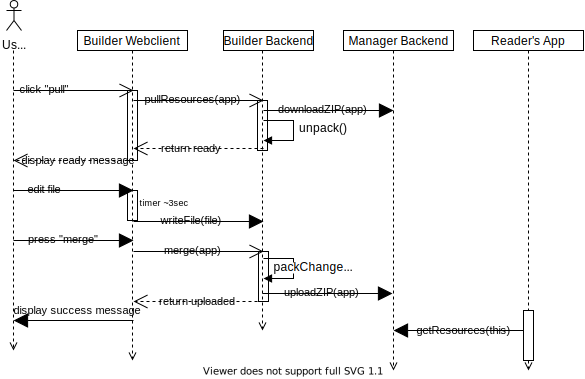
\includegraphics[width=0.9\textwidth]{pics/user-flow.uml.drawio.png}
  \caption{A typical interaction of a user with the UI Editor frontend and it's dependencies}
  \label{fig:userflow}
\end{figure}
\pagebreak
\section{Software stack}
From a company's perspective, it is advantageous to keep the technology stack as narrow as possible.
For this case study, the most important point was the availability of additional personnel with knowledge about the frameworks and languages used.
To conform with the company's \Gls{devops} practices the only requirement is to run the project inside Docker containers in a \Gls{kubernetes} environment.
\\\\
For this project the Typescript language (\url{https://www.typescriptlang.org}) is used on back- and frontend.
The advantage is the availability of many skilled personnel in the company as well as an established ecosystem and easy sharing of code and type definitions between frontend and backend.
\\
The rest of the software stack is fairly common in today's web development industry too:

\begin{description}
  \item[Frontend] \leavevmode
  \begin{description}
    \item[Rendering framework] \textit{React JS v18} (\url{https://reactjs.org/})
    \item[UI Component Library] \textit{Blueprint JS} (\url{https://blueprintjs.com/}) provides components so a consistent design system with common functionality like buttons, dropdowns, filters etc. can be used.
    \item[Other libraries] \textit{ReactQuery / TanQuery} to manage, cache and invalidate HTTP API requests to the backend, \textit{Zustand JS} for shared reactive state management and \textit{Zod} for type validation at runtime.
  \end{description}
  \item[Backend] \leavevmode
  \begin{description}
    \item[HTTP Server] Express on Node JS, which is the most common combination to run an JavaScript based HTTP server (see \cite{Github:VanoDevium/node-framework-stars}).
    \item[Routing abstraction] TSOA (\url{https://github.com/lukeautry/tsoa}) on top of Express, which is a Typescript library to provide Java-Spring like syntax with controllers, dependency injection and parameter validation at runtime.
  \end{description}
  \item[Testing] using Vitest (\url{https://vitest.dev/}) for Unit tests and Playwright (\url{https://playwright.dev/}) as E2E test runtime. 
  \item[DevOps] Gitlab Pipelines to build, test and package on every merge request or commit to develop and master branch.
  \item[Project Setup] Monorepository with PNPM as package manager and Turborepo to manage package dependencies and automatic optimal build scheduling and caching.
\end{description}

\section{CI/CD}

Continuous Integration and Continuous Delivery, short CI/CD, a core practice of agile software development, enables fast release and deployment cycles which is crucial for agile prototyping and development.
A Gitlab CI/CD Pipeline was set up for the UI builder, consisting of Build, Package, and Deploy stages.
The Build stage also executed unit and end-to-end tests due to technical reasons for efficiency.\\
Having a fast and reliable CI/CD process during development and prototyping was valuable, as it allowed for quick reactions to user input and deployment to a staging domain for user feedback in under 10 minutes.
Separating staging and production systems also allowed for more confident deployment of quick fixes for validation in a production-like environment without interrupting users.

\section{Feature examples}

A selection of features is presented that were implemented during the UI Editor case study is presented in the following section.
These features are chosen as examples to how the HCI methods and outcomes from the user research phase influenced their design and how they can improve the user's experience with the tool. 

\subsection{File management - open multiple files as tabs}

A common workflow consists of editing multiple files simultaneously, for example having the view configuration open while adding translations for newly added components.
The old editor tool allowed to only open one file at a time, which got closed when the user opened another file. This showed up as a big slowdown during the moderated observation.
All participants mentioned they have to work on multiple files and that they are annoyed by the workflow, especially when opening large view configs can take more than 30 seconds.
\\
The solution was inspired by the file management that most \Gls{ide}s provide; a bar on top where all the opened files are listed and the user can quickly switch between them or close the ones not needed (see fig. \ref{fig:file-tabs}). 

\begin{figure}[h!]
  \includegraphics[width=\textwidth]{pics/file_tabs.png}
  \caption{Screenshot of the latest iteration of file tabs}
  \label{fig:file-tabs}
\end{figure}

\subsection{File management - quick links}

A second feature regarding the file management is ``quick links''. While all target groups benefit from this, especially for the personas \textit{Steffi, \ref{persona:productdev}} and \textit{Karsten, \ref{persona:itpublishing}}
this can speed up common tasks considerably.

The basic idea is to bookmark commonly used files, e.g. the translation or ad config, and have them prominently available when opening a new app.
For the implementation, three factors needed to be considered:
\begin{description}
  \item[Where to save?] The quick links are stored in the \Gls{localstorage} of the user's browser, so the list is available across apps.
  \item[How to manage?] The user has a list on the settings view, where entries can be added, deleted and changed, but the file path needs to be inserted manually. To enhance the user experience, a proposal exists to either add a file picker in the settings or add a bookmark button to the file manager.
  \item[How to present the links?] The links must be easily accessible to provide the intended benefit. The solution was to show them prominently when entering the \textit{edit} view and no file was opened yet.
  In addition, the UI shows if the link points to a file, which gets opened as a new file tab, to a folder which will navigate the file explorer there, or if the path doesn't exist in the current app.
  \begin{figure}[h!]
    \centering
    \includegraphics[width=0.4\textwidth]{pics/quick_links.png}
    \caption{The three types of quick links: Folder, file and not available}
  \end{figure}
\end{description}

\subsection{Editor - Abstraction to provide per-file custom editors}

Purple Experience relies on a variety of configuration files, all with different schemata and functional intents.
To provide an efficient and error reduced workflow to users, it is important to have specialized file editors.

For view configurations for example, the JSON Editor Library (\url{https://github.com/json-editor/json-editor}) is used, combined with the generated JSON Schema files. For the translations there exists a custom editor that has a fuzzy search function and makes it easy to manage translation entries.

The abstraction is done solely in the frontend and follows React's ``\Gls{comp-over-inh}'' pattern and can be seen in fig. \ref{fig:abstract-editor}.
To add a new specialized editor the only two steps are creating a new functional component that implements the \textit{EditorImpl} interface
and add that editor in the \textit{EditorRegistry} to get returned for the file paths in question.
\begin{figure}[h!]
  \includegraphics[width=\textwidth]{pics/abstract_editor_uml.drawio.png}
  \caption{Class diagram showing the editor abstraction in React JS. Due to modern React JS architecture, component classes are replaced with functional components (marked with $\ll functional\gg$).}
  \label{fig:abstract-editor}
\end{figure}
Examples of custom editor implementations can be seen in Appendix \ref{fig:messages_editor} and \ref{fig:ads-editor}.
By implementing Editors for multiple levels of expertise, users like persona ``Karsten'' (\ref{persona:itpublishing}) can make small adaptions like changing a translation without worrying about the underlying file format and without the possibility to break the app due to syntax errors.

\section{Automated Testing}
\label{sec:automated-testing}

Automated tests contribute to the confidence of developers to deploy more frequently and can reduce load from the QA team to test common workflows over and over.
two of the most common testing levels were used for the project: unit tests and End-to-End tests (also known as E2E or System tests).
\\\\
Unit tests test one ``component'' in a sandboxed environment, in practice often done per-function or per-class.
On the client, both UI components and business logic code that is encapsulated in classes or JavaScript modules get tested.

They also enable Test-driven development, where the tests are written upfront based on specifications and constraints with invariants, pre- and postconditions and the code is continously tested against them.
\\
For agile development, the speed of the test execution and CI/CD Pipelines is important. The developer is usually blocked during that time and can't progress on the task.
Therefore, the aim was to find a fast runtime, compatible with UI- / browser testing as well as Node JS for the server code.
After evaluating commonly used frameworks, Vitest \footnote{\url{https://vitest.dev/}} was chosen as a test framework which fullfills all the requirements. Tests can be hot-reloaded and re-executed on change in less than a second, providing a good developer experience.
\\\\
Due to the complexity of interoperation between components, APIs and the Web standards, unit tests alone are not enough to guarantee the different modules work together as expected. 
\\
E2E tests are supposed to cover a typical user interaction with the service to validate the interaction between business logic components, UI and the user itself.
First a headless browser\footnote{Headless browsers are browser instances that don't render the actual content to a user's screen, but run as a CLI application and still execute all JavaScript, CSS and HTML.} (\url{https://pptr.dev/}) was used in combination with Vitest,
but writing and debugging tests proved to be slow and error-prone.
\\\\
Later in the process, the E2E tests were rewritten for an alternative test framework called Playwright (\url{https://playwright.dev/}), which allows recording a test case in a normal browser window and then generates the test code automatically, allowing to be adapted and generalized if needed.
After the tests were ported to the new framework developers can enjoy better debugging tools and the ability to add new tests easier.
\\
This can be an example for others, that investing time to investigate new tools and port code to them if they bring value can improve developer experience and thus also speed and confidence.

\section{Privacy-friendly analytics \& monitoring}
\label{sec:analytics}

Sooner or later, you find yourself in a pickle when it comes to tracking.
On the one hand, the data can provide valuable insights into the behavior of many users, which would not be possible through qualitative research.
On the other hand, the most common tools like Google Analytics track users with cookies, which creates new challenges regarding GDPR compliance.
\\\\
The Purple product owner showed me a SaaS called \url{https://squeaky.ai/}, which is a cookieless solution to track users on this page.
While it can't provide the same level of demographic information a cookie based solution can, it still collects the most important data like usage statistics,
user interactions, occurred JavaScript errors and can even show heatmaps per page to visualize which UI elements the user interacts with the most.

\begin{figure}[h]
  \centering
  \includegraphics[width=0.75\textwidth]{pics/squeaky_heatmap.jpg}
  \caption{Screenshot: Squeaky.ai heatmap of an app's edit view}
  \label{fig:squeaky}
\end{figure}

These heatmaps for example can show if a new UI feature is used by users and how they interact with the page in general.
Fig. \ref{fig:squeaky} shows that the users mostly interacted with the file explorer and only did a few clicks in the editor panel.

To analyze the usage growth, fig. \ref{fig:squeaky_users} indicates how the number of page views per week increased steadily since the internal beta was launched (except for the dip during the Christmas holidays).
The graph clearly shows that the time-bound goal from the SMART goals (\ref{fig:smart}) has been successfully achieved.

\begin{figure}[h]
  \centering
  \includegraphics[width=\textwidth]{pics/squeaky_user_curve.jpg}
  \caption{Screenshot: Squeaky.ai page views since December 2022}
  \label{fig:squeaky_users}
\end{figure}

\section{User Testing, Feedback, Beta and Monitoring}

After a first stable deployment was available for stating and production dynamic resources and all basic requirements were met, the user tests for the Beta-phase started.
Four people from our company agreed to try to use the editor and give verbal feedback. Three of them were already participants of the interviews and they covered all mayor groups of users,
so the feedback represented all different expertise levels.

The reported bugs were and still will be written into Jira tickets so the status can be properly tracked and release notes can be easier generated.
Mostly the bugs were edge cases where a file wouldn't open or the changes were not saved properly.


\section{Communication and Documentation}
Communicating with the test users and documenting the technical aspects of the software, the progress and how to use certain features is
another building block towards a good user- and developer experience.
\subsection{Asynchronous communication}
For the asynchronous communication, a Microsoft Teams Channel was utilized, a group chat where all invited persons (in case of the internal Beta-phase company-wide) can write with each other and create posts.
This was used for notifications about new deployments and if in the aftermath someone found a bug that could affect multiple people.

Even though this adds a bit overhead, it proved easier than having everyone write bug tickets directly, as user often don't know how to describe the problem which leads to unclear descriptions, wrong tags and duplicate tickets.
Instead, a developer with knowledge about the system looked at the reports and created a new ticket if the problem was new, otherwise referenced an existing ticket or forwarded the problem to the responsible team.
Jira tickets were all assigned to the UI builder component as well as specific releases so everyone can see with one click which changes and fixes are contained in which release.

\subsection{Presentation and Beta kickoff}
At the point where the company-wide beta phase started, a presentation meeting was scheduled where I first explained the project,
demonstrated a common work flow and some of the most important features and could directly respond to questions or feedback.
Around 30 employees attended, including quality assurance and customer success managers, covering a wide range of people who possibly will come in touch with the tool.

\subsection{Documentation}
For the feature documentation, Sprylab uses Confluence for internal documentation and Archbee for external documentation that customers can access too.
As we have the common problem of documentation getting postponed indefinitely, I tried to integrate writing documentation directly int o the development flow and only close a ticket if the documentation
was written and reviewed by one additional person. Due to time and personnel shortages, this was unfortunately not always possible and will require more future attention.


% ---------------------------------------------------
% ----- Conclusion of the template
% ----- for Bachelor-, Master thesis and class papers
% ---------------------------------------------------
%  Created by C. Müller-Birn on 2012-08-17, CC-BY-SA 3.0.
%  Freie Universität Berlin, Institute of Computer Science, Human Centered Computing. 
%
\chapter{Conclusion and outlook}
\label{chap:conclusion}      
In conclusion, this thesis has demonstrated the challenges and opportunities of applying HCI principles and methods in a brownfield software development project through the redevelopment of a UI editor for a digital publishing company, Sprylab.
During the process, I have shown how common user research methods can be adapted them for this specific case study.
Agile development and Lean UX enabled to iterate quickly with new ideas and archive fast deployments to a staging system.
With a growing group of users already using the software in production and the majority of feedback positive, I'm confident that this new software is a stable and extensible tool, especially regarding the two factors Usability and Time-on-Task.
\\\\
However, there is still room for improvements in terms of accessibility and entry hurdle for new users.
The entry hurdle is still high and a lot of background knowledge is assumed, which is partly due to the complexity of other systems in the ecosystem that were set as technical requirements from the beginning on.
Moving forward, replacing the JSON editor with a custom implementation that combines JSON schemata and generated UI is one of the next steps, which will speed up the user's
workflow even more and allow for further improvements that are impossible with a third-party library.
\\\\
Overall, this thesis has demonstrated the importance of considering HCI principles and methods in brownfield software development projects, and the potential benefits that can be achieved when these approaches are applied in a real-world context.


%---------------------------------------------------
%----- Bibliography
%---------------------------------------------------
\phantomsection
\addcontentsline{toc}{chapter}{Literatur}
% \bibliographystyle{alpha}
\printbibliography



%---------------------------------------------------
%----- Appendix   
%---------------------------------------------------
\backmatter
\printnoidxglossaries
% ---------------------------------------------------
% ----- Appendix of the template
% ----- for Bachelor-, Master thesis and class papers
% ---------------------------------------------------
%  Created by C. Müller-Birn on 2012-08-17, CC-BY-SA 3.0.
%  Freie Universität Berlin, Institute of Computer Science, Human Centered Computing. 
%

\chapter{Appendix}
\label{ch:Appendix}

\section{Personas}
\label{app:personas}


% Persona 1
\subsection{John - Purple Experience Product Developer}
\label{subsec:persona:productdev}
\subsubsection{Background and Skills}
John (34) is a senior Angular Web Developer at Sprylab, working there for two years. He was born in Berlin and lives in Lichterfelde with his wife and mostly works from home. He is passionate about Angular, Typescript and Developer Experience in general, studied Computer Science at the Beuth Hochschule and hosts Angular conferences.
\\
\subsubsection{Goals and work with the Editor}
\begin{itemize}
  \item Test newly developed features and the related configurations
  \item Configure test apps for development and QA purposes
  \item Support in case Project Developers like <TODO> encounter problems
  \item John works with the editor multiple times a week
\end{itemize}

\hrule
% Persona 2
\subsection{Steffi - Project Developer}
\label{subsec:persona:projectdev}
\subsubsection{Background and Skills}
Steffi (23) studies media informatics and works as a working student at Sprylab since a year. This is her first job in the industry and she is learning new things every day. Her skills include writing CSS and understanding modern web technologies, but she still struggles using native and custom debugging tools if something goes wrong.  
\\
\subsubsection{Goals and work with the Editor}
\begin{itemize}
  \item Configure new apps based on existing templates and adapt them to customer's requirements
  \item Add new components or change data sources for existing apps
  \item Add custom HTML pages or Javascript snippets to intergrate external services
  \item Change styles, color schemas or icons when a customer has a rebranding
  \item Steffi uses the editor as a primary tool for her work
\end{itemize}

\hrule
% Persona 2
\subsection{Karsten - IT department at a publishing house}
\label{subsec:persona:itpublishing}
\subsubsection{Background and Skills}
Karsten (46) worked in the publishing industry for 20 years, but only during the last years his company, aga magazine publisher, tries to catch up with the digital development and trends. He is still struggling with his role and is thankful for every trick or tool that makes his life managing the digital products easier.
\\
\subsubsection{Goals and work with the Editor}
\begin{itemize}
  \item Exchange logos and colors when the magazines he supervies get a redesign
  \item Add new ads to different views when a new campaign starts
  \item Manage URLs to external sites when they change
  \item Karsten uses the Editor once a month on average
\end{itemize}


\section{Zweiter Teil Appendix}
\label{app:second_appendix}  



\end{document}